\section{Results: diffuse scattering and stacking disorder in PbI\texorpdfstring{$_2$}{2}}
\label{sec:results_pbi2}

Figure~\ref{fig:pbi2_diffuse_cylinders} shows a CVD-grown PbI$_2$ film and a crop spanning the $r=0$ and $r=1$ reciprocal rods. The $r=1$ rod contains measurable intensity between the integer Bragg maxima, whereas the $r=0$ rod is dominated by sharp peaks and finite-thickness oscillations. This rod-dependent redistribution is the experimental motivation for the stacking-disorder model. In a two-dimensional powder, random in-plane orientation maps each $(h,k)$ rod onto a reciprocal-space cylinder at fixed $Q_R$. An infinite ordered crystal gives intensity at discrete crystallite-frame $L$ values, while a finite ordered stack already produces a continuous $S_{hk}(L)$ with finite widths and fringes. Stacking faults do not create these rods. They change the correlations among trilayers and redistribute intensity within the existing continuous rod profile.

\begin{figure}[H]
  \centering
  \begin{minipage}{0.78\linewidth}
    \centering
    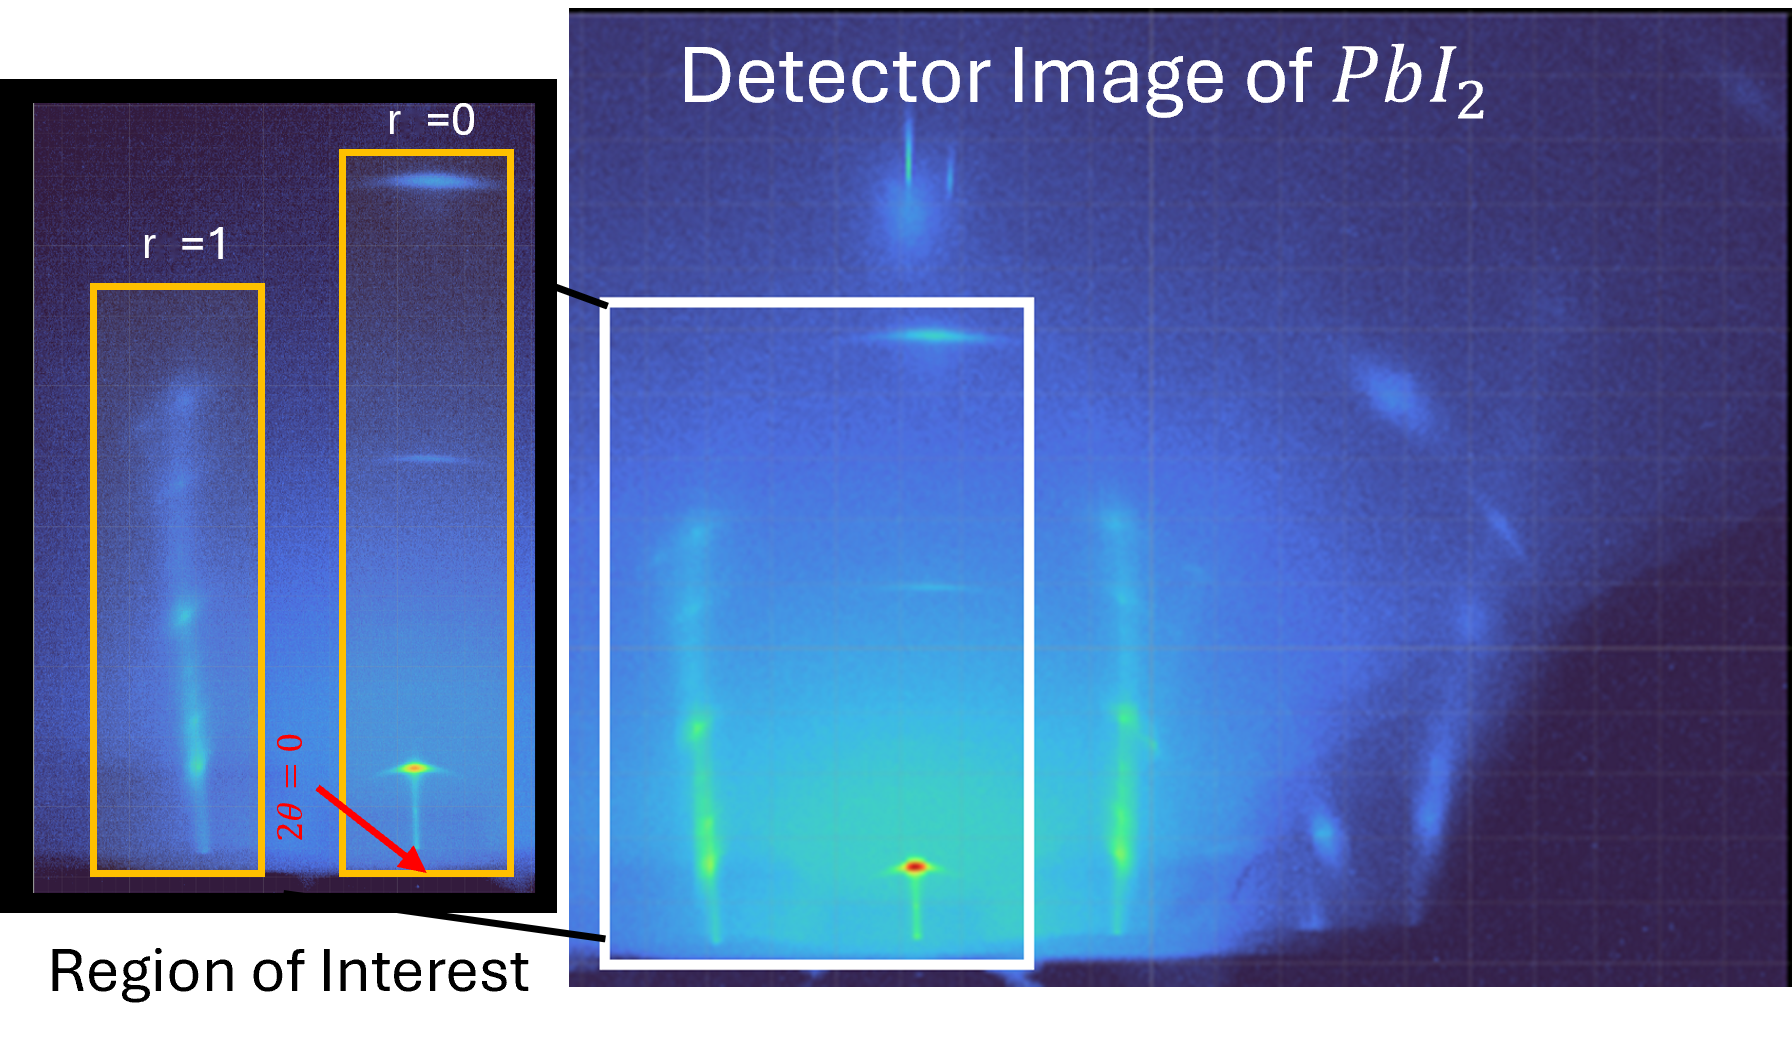
\includegraphics[width=\linewidth]{figures/results_pbi2/PbI2_detector.png}
  \end{minipage}
  \caption{Measured PbI$_2$ diffraction image (right) and an enlarged region of interest (left). The direct-beam position defines the vertical $r=0$ trajectory. Diffuse intensity is visible between the ordered maxima on the neighboring $r=1$ rod, while the $r=0$ profile is contrast-matched to the basal-plane shifts included in the stacking model.}
  \label{fig:pbi2_diffuse_cylinders}
\end{figure}

The contrast between the two rods identifies the structural information carried by the diffuse intensity. A forward basal-plane shift $\mathbf s=(1/3,2/3)$ multiplies the amplitude of one $(h,k)$ rod by
\begin{equation}
  \omega_{hk}=\exp\!\left[2\pi i(hs_x+ks_y)\right]
  =\exp\!\left[\frac{2\pi i}{3}(h+2k)\right].
  \label{eq:pbi2_registry_phase}
\end{equation}
For $h=k=0$, $\omega_{00}=1$, and the two trilayer orientations have the same $00L$ amplitude in the present model. The $r=0$ rod is therefore insensitive to the included basal-plane shifts and orientation changes: faults can be present, but they are contrast-matched on that rod. Off-specular rods retain the lateral phase contrast, so the same faults change their pair interference and transfer intensity from ordered maxima into the diffuse regions between them.

\subsection{From stacking faults to rod intensity}
\label{sec:pbi2_transition_model}

The structural unit is one I--Pb--I trilayer. Its state is described by a basal-plane position $\rho\in\{0,1,2\}$ and an orientation $\sigma\in\{+,-\}$. The ordered 2H, 4H, and 6H parents are deterministic sequences of these six possible layer states. Figure~\ref{fig:pbi2_transition_states} renders the corresponding cycles as projected I--Pb--I stacks. Read from bottom to top, they are $0F_+\rightarrow0F_+$ for 2H, $0F_+\rightarrow1F_-\rightarrow0F_+$ for 4H, and $0F_+\rightarrow1F_+\rightarrow2F_+\rightarrow0F_+$ for 6H. The existence and crystallographic stacking sequences of these parent polytypes are established experimentally.\cite{Minagawa1975,Palosz1990}

\begin{figure}[H]
  \centering
  \resizebox{0.88\linewidth}{!}{%
    % PbI2 polytype-stack schematic rendered directly by main.tex.
% Required packages/libraries are loaded in the manuscript preamble:
% tikz, xcolor, and the calc and arrows.meta TikZ libraries.
\begingroup

\definecolor{iodine}{RGB}{145,20,145}
\definecolor{lead}{RGB}{74,76,82}
\definecolor{guideblue}{RGB}{0,105,145}
\definecolor{guidegreen}{RGB}{55,175,35}
\definecolor{chargecyan}{RGB}{0,205,225}

\tikzset{
	cell edge/.style={
		draw=black!70,
		line width=0.45pt
	},
	blue guide/.style={
		draw=guideblue,
		line width=0.65pt,
		dash pattern=on 2.3pt off 2.0pt
	},
	green guide/.style={
		draw=guidegreen,
		line width=0.65pt,
		dash pattern=on 2.3pt off 2.0pt
	},
	bracket/.style={
		draw=black,
		line width=0.75pt,
		line cap=round,
		line join=round
	},
	panel title/.style={
		font=\sffamily\bfseries\fontsize{13}{14}\selectfont,
		text=black!85
	},
	stack label/.style={
		font=\sffamily\bfseries\fontsize{14}{15}\selectfont,
		text=black!80
	}
}

% Pb--I bond: dark outer cylinder, gray Pb half, violet I half.
\newcommand{\PbIbond}[2]{%
	\draw[
	black!72,
	line width=1.55pt,
	line cap=round
	] (#1) -- (#2);
	
	\draw[
	lead!92,
	line width=0.86pt,
	line cap=round
	] (#1) -- ($(#1)!0.53!(#2)$);
	
	\draw[
	iodine!95,
	line width=0.86pt,
	line cap=round
	] ($(#1)!0.47!(#2)$) -- (#2);
}

\newcommand{\Iatom}[1]{%
	\shade[ball color=iodine]
	(#1) circle[radius=13];
	
	\draw[
	black!55,
	line width=0.22pt
	] (#1) circle[radius=13];
}

\newcommand{\Pbatom}[1]{%
	\shade[ball color=lead]
	(#1) circle[radius=18];
	
	\draw[
	black!60,
	line width=0.25pt
	] (#1) circle[radius=18];
}

% Coordinates for an A layer.
% #1 = coordinate prefix.
% #2 = y coordinate of the upper iodine row.
\newcommand{\NormalAcoords}[2]{%
	\coordinate (#1T1) at (174,{#2});
	\coordinate (#1T2) at (273,{#2});
	\coordinate (#1T3) at (372,{#2});
	
	\coordinate (#1P1) at (239,{#2+47});
	\coordinate (#1P2) at (338,{#2+47});
	
	\coordinate (#1B1) at (207,{#2+93});
	\coordinate (#1B2) at (305,{#2+93});
	\coordinate (#1B3) at (404,{#2+93});
}

% Coordinates for a B layer.
\newcommand{\Bcoords}[2]{%
	\coordinate (#1T1) at (207,{#2});
	\coordinate (#1T2) at (305,{#2});
	
	\coordinate (#1P) at (273,{#2+47});
	
	\coordinate (#1B1) at (239,{#2+93});
	\coordinate (#1B2) at (338,{#2+93});
}

% B layer flipped about its fixed Pb position.
\newcommand{\Binvcoords}[2]{%
	\coordinate (#1T1) at (239,{#2});
	\coordinate (#1T2) at (338,{#2});
	
	\coordinate (#1P) at (273,{#2+47});
	
	\coordinate (#1B1) at (207,{#2+93});
	\coordinate (#1B2) at (305,{#2+93});
}

\newcommand{\DrawNormalA}[1]{%
	\PbIbond{#1P1}{#1T1}
	\PbIbond{#1P1}{#1T2}
	\PbIbond{#1P1}{#1B1}
	\PbIbond{#1P1}{#1B2}
	
	\PbIbond{#1P2}{#1T2}
	\PbIbond{#1P2}{#1T3}
	\PbIbond{#1P2}{#1B2}
	\PbIbond{#1P2}{#1B3}
	
	\Iatom{#1T1}
	\Iatom{#1T2}
	\Iatom{#1T3}
	
	\Iatom{#1B1}
	\Iatom{#1B2}
	\Iatom{#1B3}
	
	\Pbatom{#1P1}
	\Pbatom{#1P2}
}

\newcommand{\DrawB}[1]{%
	\PbIbond{#1P}{#1T1}
	\PbIbond{#1P}{#1T2}
	\PbIbond{#1P}{#1B1}
	\PbIbond{#1P}{#1B2}
	
	\Iatom{#1T1}
	\Iatom{#1T2}
	
	\Iatom{#1B1}
	\Iatom{#1B2}
	
	\Pbatom{#1P}
}

\newcommand{\DrawBinv}[1]{%
	\PbIbond{#1P}{#1T1}
	\PbIbond{#1P}{#1T2}
	\PbIbond{#1P}{#1B1}
	\PbIbond{#1P}{#1B2}
	
	\Iatom{#1T1}
	\Iatom{#1T2}
	
	\Iatom{#1B1}
	\Iatom{#1B2}
	
	\Pbatom{#1P}
}

	\begin{tikzpicture}[x=0.1mm,y=-0.1mm]
		
		% Compact two-column layout:
		% 2H above 4H on the left.
		% 2H monolayer above 6H on the right.
		\path[use as bounding box]
		(0,0) rectangle (900,990);
		
		% ================================================================
		% Top left: 2H
		% ================================================================
		\begin{scope}[shift={(-40,0)}]
			
			\node[panel title] at (289,18) {(a) 2H};
			
			\NormalAcoords{hU}{60}
			\NormalAcoords{hL}{225}
			
			% Projected unit-cell edges.
			\draw[cell edge]
			(hUP1) -- (hUP2);
			
			\draw[cell edge]
			(hUP1) -- (hLP1);
			
			\draw[cell edge]
			(hUP2) -- (hLP2);
			
			\draw[cell edge]
			(hLP1) -- (hLP2);
			
			\DrawNormalA{hU}
			\DrawNormalA{hL}
			
			% Registry guides.
			\draw[green guide]
			(239,60) -- (239,355);
			
			\draw[green guide]
			(272,60) -- (272,355);
			
			\draw[green guide]
			(306,60) -- (306,355);
			
			\draw[green guide]
			(338,60) -- (338,355);
			
			\draw[blue guide]
			(174,225) -- (405,225);
			
			\draw[blue guide]
			(239,272) -- (386,272);
			
			\draw[blue guide]
			(207,318) -- (418,318);
			
			% Restore the rightmost lower iodine above the dashed guide.
			\Iatom{hLB3}
			
			% Ionic signs on the reference A layer.
			\foreach \a in {hLT1,hLT2,hLT3,hLB1,hLB2,hLB3}{
				\node[
				text=chargecyan,
				font=\bfseries\fontsize{9}{9}\selectfont
				] at (\a) {$-$};
			}
			
			\foreach \a in {hLP1,hLP2}{
				\node[
				text=guidegreen!85!black,
				font=\bfseries\fontsize{9}{9}\selectfont
				] at (\a) {$+$};
			}
			
			% Layer brackets.
			\draw[bracket]
			(150,60)
			-- (134,60)
			-- (134,153)
			-- (150,153);
			
			\draw[bracket]
			(150,225)
			-- (134,225)
			-- (134,318)
			-- (150,318);
			
			% Stacking labels.
			\node[stack label] at (98,107)
			{$0F_{+}$};
			
			\node[stack label] at (98,272)
			{$0F_{+}$};
			
		\end{scope}
		
		% ================================================================
		% Bottom left: 4H
		% ================================================================
		\begin{scope}[shift={(-40,385)}]
			
			\node[panel title] at (289,18) {(c) 4H};
			
			\Binvcoords{fU}{60}
			\NormalAcoords{fL}{225}
			
			% Projected unit-cell edges.
			\draw[cell edge]
			(239,107) -- (338,107);
			
			\draw[cell edge]
			(239,107) -- (fLP1);
			
			\draw[cell edge]
			(338,107) -- (fLP2);
			
			\draw[cell edge]
			(fLP1) -- (fLP2);
			
			\DrawBinv{fU}
			\DrawNormalA{fL}
			
			% Registry guides.
			\draw[green guide]
			(239,60) -- (239,355);
			
			\draw[green guide]
			(272,60) -- (272,355);
			
			\draw[green guide]
			(306,60) -- (306,355);
			
			\draw[green guide]
			(338,60) -- (338,355);
			
			\draw[blue guide]
			(174,225) -- (405,225);
			
			\draw[blue guide]
			(239,272) -- (386,272);
			
			\draw[blue guide]
			(207,318) -- (418,318);
			
			% Restore the rightmost lower iodine above the dashed guide.
			\Iatom{fLB3}
			
			% Ionic signs on the reference A layer.
			\foreach \a in {fLT1,fLT2,fLT3,fLB1,fLB2,fLB3}{
				\node[
				text=chargecyan,
				font=\bfseries\fontsize{9}{9}\selectfont
				] at (\a) {$-$};
			}
			
			\foreach \a in {fLP1,fLP2}{
				\node[
				text=guidegreen!85!black,
				font=\bfseries\fontsize{9}{9}\selectfont
				] at (\a) {$+$};
			}
			
			% Layer brackets.
			\draw[bracket]
			(150,60)
			-- (134,60)
			-- (134,153)
			-- (150,153);
			
			\draw[bracket]
			(150,225)
			-- (134,225)
			-- (134,318)
			-- (150,318);
			
			% Stacking labels.
			\node[stack label] at (93,107)
			{$1F_{-}$};
			
			\node[stack label] at (98,272)
			{$0F_{+}$};
			
		\end{scope}
		
		% ================================================================
		% Top right: single A layer of 2H
		% ================================================================
		\begin{scope}[shift={(420,0)}]
			
			\node[panel title] at (289,18)
			{(b) $F_{+}$ trilayer};
			
			\NormalAcoords{m}{65}
			
			% Projected in-plane cell edge.
			\draw[cell edge]
			(mP1) -- (mP2);
			
			\DrawNormalA{m}
			
			% Reference guides and labels appear only in this panel.
			\draw[green guide]
			(239,65) -- (239,205);
			
			\draw[green guide]
			(272,65) -- (272,205);
			
			\draw[green guide]
			(306,65) -- (306,205);
			
			\draw[green guide]
			(338,65) -- (338,205);
			
			\draw[blue guide]
			(174,65) -- (405,65);
			
			\draw[blue guide]
			(239,112) -- (386,112);
			
			\draw[blue guide]
			(207,158) -- (418,158);
			
			% Restore the rightmost lower iodine above the dashed guide.
			\Iatom{mB3}
			
			% Ionic signs.
			\foreach \a in {mT1,mT2,mT3,mB1,mB2,mB3}{
				\node[
				text=chargecyan,
				font=\bfseries\fontsize{9}{9}\selectfont
				] at (\a) {$-$};
			}
			
			\foreach \a in {mP1,mP2}{
				\node[
				text=guidegreen!85!black,
				font=\bfseries\fontsize{9}{9}\selectfont
				] at (\a) {$+$};
			}
			
			% Atomic-plane labels.
			\node[
			anchor=west,
			font=\fontsize{11}{12}\selectfont
			] at (400,65) {$\mathrm{I}_{2}$};
			
			\node[
			anchor=west,
			font=\fontsize{11}{12}\selectfont
			] at (379,114) {$\mathrm{Pb}$};
			
			\node[
			anchor=west,
			font=\fontsize{11}{12}\selectfont
			] at (425,160) {$\mathrm{I}_{1}$};
			
			% In-plane phase axis aligned with the green registry guides.
			\draw[black!70,line width=0.45pt]
			(239,210) -- (338,210);
			
			\foreach \x/\lab in {239/{$0$},272/{$\displaystyle\frac{\pi}{3}$},306/{$\displaystyle\frac{2\pi}{3}$},338/{$\pi$}}{
				\draw[black!70,line width=0.45pt] (\x,207) -- (\x,213);
				\node[
				font=\fontsize{6.5}{7}\selectfont,
				anchor=north east,
				rotate=65
				] at (\x,216) {\lab};
			}
			
			\node[
			font=\fontsize{7}{8}\selectfont,
			anchor=west
			] at (347,210) {registry phase};

		\end{scope}
		
		% ================================================================
		% Bottom right: 6H
		% ================================================================
		\begin{scope}[shift={(420,335)}]
			
			\node[panel title] at (289,18) {(d) 6H};
			
			\NormalAcoords{sU}{50}
			\NormalAcoords{sL}{500}
			
			% C layer.
			\coordinate (sCT1) at (239,200);
			\coordinate (sCT2) at (339,200);
			
			\coordinate (sCP) at (305,247);
			
			\coordinate (sCB1) at (273,293);
			\coordinate (sCB2) at (371,293);
			
			% B layer.
			\Bcoords{sM}{350}
			
			% Projected unit-cell edges.
			\draw[cell edge]
			(sUP1) -- (sUP2);
			
			\draw[cell edge]
			(sUP1) -- (sLP1);
			
			\draw[cell edge]
			(sUP2) -- (sLP2);
			
			\draw[cell edge]
			(sLP1) -- (sLP2);
			
			% Top A layer.
			\DrawNormalA{sU}
			
			% C layer.
			\PbIbond{sCP}{sCT1}
			\PbIbond{sCP}{sCT2}
			\PbIbond{sCP}{sCB1}
			\PbIbond{sCP}{sCB2}
			
			\Iatom{sCT1}
			\Iatom{sCT2}
			\Iatom{sCB1}
			\Iatom{sCB2}
			
			\Pbatom{sCP}
			
			% B and lower A layers.
			\DrawB{sM}
			\DrawNormalA{sL}
			
			% Registry guides.
			\draw[green guide]
			(272,50) -- (272,625);
			
			\draw[green guide]
			(306,50) -- (306,625);
			
			\draw[green guide]
			(239,547) -- (239,625);
			
			\draw[green guide]
			(338,547) -- (338,625);
			
			\draw[blue guide]
			(174,500) -- (405,500);
			
			\draw[blue guide]
			(239,547) -- (386,547);
			
			\draw[blue guide]
			(207,593) -- (418,593);
			
			% Restore the rightmost lower iodine above the dashed guide.
			\Iatom{sLB3}
			
			% Ionic signs on the reference A layer.
			\foreach \a in {sLT1,sLT2,sLT3,sLB1,sLB2,sLB3}{
				\node[
				text=chargecyan,
				font=\bfseries\fontsize{9}{9}\selectfont
				] at (\a) {$-$};
			}
			
			\foreach \a in {sLP1,sLP2}{
				\node[
				text=guidegreen!85!black,
				font=\bfseries\fontsize{9}{9}\selectfont
				] at (\a) {$+$};
			}
			
			% Layer brackets.
			\draw[bracket]
			(150,50)
			-- (134,50)
			-- (134,143)
			-- (150,143);
			
			\draw[bracket]
			(158,200)
			-- (142,200)
			-- (142,293)
			-- (158,293);
			
			\draw[bracket]
			(164,350)
			-- (147,350)
			-- (147,443)
			-- (164,443);
			
			\draw[bracket]
			(150,500)
			-- (134,500)
			-- (134,593)
			-- (150,593);
			
			% Stacking labels.
			\node[stack label] at (98,97)
			{$0F_{+}$};
			
			\node[stack label] at (98,247)
			{$2F_{+}$};
			
			\node[stack label] at (98,397)
			{$1F_{+}$};
			
			\node[stack label] at (98,547)
			{$0F_{+}$};
			
		\end{scope}
		
		% ================================================================
		% One shared lattice-direction axis
		% ================================================================
		% Since y=-0.1mm, decreasing y points visually upward.
		\coordinate (Oax) at (28,965);
		
		\draw[
		-{Latex[length=2.2mm,width=1.6mm]},
		line width=0.8pt
		]
		(Oax) -- ++(0,-52)
		node[
		above,
		font=\sffamily\fontsize{10}{10}\selectfont
		] {$c$};
		
		\draw[
		-{Latex[length=2.2mm,width=1.6mm]},
		line width=0.8pt
		]
		(Oax) -- ++(52,0)
		node[
		right,
		font=\sffamily\fontsize{10}{10}\selectfont
		] {$a$};
		
	\end{tikzpicture}
	
\endgroup
%
  }
  \caption{Deterministic PbI$_2$ parent cycles used in the transition model. (a) 2H repeats $0F_+$. (b) The isolated $F_+$ trilayer defines the local orientation. (c) 4H alternates $0F_+$ and $1F_-$. (d) 6H advances $0F_+\rightarrow1F_+\rightarrow2F_+\rightarrow0F_+$. In a state label $\rho F_\sigma$, $\rho$ is the basal-plane position and $\sigma$ is the trilayer orientation.}
  \label{fig:pbi2_transition_states}
\end{figure}

Adjacent trilayers are connected by five allowed interface events. The event $a$ leaves the basal-plane position and orientation unchanged. The events $b_+$ and $b_-$ shift the next trilayer forward or backward without changing its orientation, while $d_+$ and $d_-$ combine those shifts with an orientation change. A change of orientation without a basal-plane shift is excluded. The parent events are $a$ for 2H, $d_+$ for 4H, and $b_+$ for 6H. Reversing the shift direction gives the symmetry-related handed counterparts.

A stacking fault is represented as a local departure from the selected parent event. For a parent-rich population $j\in\{2H,4H,6H\}$, the equal-alternative template is
\begin{equation}
  p_j(\text{parent event})=1-\epsilon_j,
  \qquad
  p_j(\text{each alternative})=\frac{\epsilon_j}{4}.
  \label{eq:pbi2_fault_parameterization}
\end{equation}
Thus $\epsilon_j$ is the effective per-interface probability of departing from the selected parent event under this template. It is not a universal PbI$_2$ fault density. The transition matrix propagates these events over multiple layer separations and calculates the phase-weighted pair correlation for each $(h,k)$ rod. The complete six-state construction, its exact rod-dependent reduction, and the finite-stack derivation are given in the Supporting Information.\cite{HendricksTeller1942,KakinokiKomura1954,KakinokiKomura1965,Hart2018}

The main physical quantity is the correlation between trilayers separated by $\Delta$ interfaces. Let $C_{hk}^{(j)}(\Delta;L,\lambda_s)$ be the disorder-averaged scattering correlation, averaged over all layer pairs at that separation, for population $j$. Let $N$ be the number of trilayers, $d$ their normal separation, and $q_z=2\pi L/c$ the crystallite-frame momentum-transfer component along the rod. The corresponding finite-stack rod intensity can be written as
\begin{equation}
  S_{hk}^{(j)}(L,\lambda_s)
  =S_{\mathrm{self},hk}^{(j)}(L,\lambda_s)
  +\frac{2}{N}\operatorname{Re}\sum_{\Delta=1}^{N-1}
  (N-\Delta)C_{hk}^{(j)}(\Delta;L,\lambda_s)e^{iq_zd\Delta}.
  \label{eq:pbi2_pair_correlation_intensity}
\end{equation}
The first term is the intensity scattered by the individual trilayers. The second is their interference, grouped by separation $\Delta$. An ordered parent preserves a periodic correlation over long separations and gives sharp maxima with finite-stack fringes. Fault events dephase or shorten that periodic correlation and transfer intensity into the diffuse regions between the maxima.

The 2H-, 4H-, and 6H-rich populations are treated as mutually incoherent, so their intensities are combined as
\begin{equation}
  S_{hk}(L,\lambda_s)=
  \sum_{j\in\{2H,4H,6H\}}w_jS_{hk}^{(j)}(L,\lambda_s),
  \qquad w_{2H}+w_{4H}+w_{6H}=1.
  \label{eq:pbi2_population_sum}
\end{equation}
This population-weighted $S_{hk}(L,\lambda_s)$ replaces the ordered finite-stack rod intensity introduced in Sec.~\ref{sec:structure_factor}. The subsequent powder-cylinder formation, mosaic broadening, Ewald selection, optical weighting, detector mapping, and finite-region integration are unchanged. The stacking model is therefore a structural module within the same detector-space forward calculation rather than a separate diffraction framework.

\subsection{Hierarchy of stacking-disorder models}
\label{sec:pbi2_model_hierarchy}

The selected comparisons should be organized as a nested model hierarchy rather than as a generic low-to-high disorder series. The first stage establishes a nearly ordered 2H baseline. The second asks whether faults within a 2H-rich population alone reproduce the diffuse redistribution. The third adds a 6H-rich population, and the fourth adds a 4H-rich population. Each stage must use the same detector geometry, background treatment, integration regions, and ordered baseline, and added complexity is retained only when it improves the fault-sensitive rod profiles without degrading the ordered maxima.

\begin{figure}[H]
  \centering
  {\large\bfseries Hierarchy of PbI$_2$ stacking-disorder models\par}
  \vspace{0.7em}
  \begin{minipage}[t]{0.48\linewidth}
    \centering\textbf{(a) 2H with little disorder}\par\vspace{0.4em}
    \fbox{\begin{minipage}[c][0.18\textheight][c]{0.92\linewidth}\centering
      Direct detector image and matched rod profile\\[0.5em]
      $\epsilon_{2H}\approx0$, $w_{2H}=1$\\[0.5em]
      Placeholder for retained arrays
    \end{minipage}}
  \end{minipage}\hfill
  \begin{minipage}[t]{0.48\linewidth}
    \centering\textbf{(b) 2H with general stacking disorder}\par\vspace{0.4em}
    \fbox{\begin{minipage}[c][0.18\textheight][c]{0.92\linewidth}\centering
      Direct detector image and matched rod profile\\[0.5em]
      $\epsilon_{2H}$ released, $w_{2H}=1$\\[0.5em]
      Placeholder for retained arrays
    \end{minipage}}
  \end{minipage}

  \vspace{1.0em}

  \begin{minipage}[t]{0.48\linewidth}
    \centering\textbf{(c) 2H + 6H disorder}\par\vspace{0.4em}
    \fbox{\begin{minipage}[c][0.18\textheight][c]{0.92\linewidth}\centering
      Direct detector image and matched rod profile\\[0.5em]
      $w_{2H}+w_{6H}=1$\\[0.5em]
      Placeholder for retained arrays
    \end{minipage}}
  \end{minipage}\hfill
  \begin{minipage}[t]{0.48\linewidth}
    \centering\textbf{(d) 2H + 6H + 4H disorder}\par\vspace{0.4em}
    \fbox{\begin{minipage}[c][0.18\textheight][c]{0.92\linewidth}\centering
      Direct detector image and matched rod profile\\[0.5em]
      $w_{2H}+w_{6H}+w_{4H}=1$\\[0.5em]
      Placeholder for retained arrays
    \end{minipage}}
  \end{minipage}
  \caption{Planned matched comparisons for a nested hierarchy of PbI$_2$ stacking-disorder models. (a) Nearly ordered 2H establishes the finite-stack baseline. (b) Faulted 2H tests whether one parent-rich population accounts for the diffuse redistribution. (c) A 6H-rich population is added to the 2H model. (d) A 4H-rich population is then added to the 2H+6H model. Every stage will use the same detector projection, background treatment, and intensity normalization. The panels remain placeholders until the direct measured and calculated arrays are inserted.}
  \label{fig:pbi2_disorder_hierarchy}
\end{figure}

\subsection{Connection to the detector calculation}
\label{sec:pbi2_detector_connection}

The stacking parameters are introduced only after detector geometry, sample alignment, mosaicity, lattice constants, and the ordered PbI$_2$ rod intensity have been fixed by the ordered-film analysis. The core parameters are the departure probabilities $\epsilon_{2H}$, $\epsilon_{4H}$, and $\epsilon_{6H}$, the normalized population weights $w_{2H}$, $w_{4H}$, and $w_{6H}$, and the finite stack length $N$. Measured and calculated detector images are projected through identical constant-$Q_R$ masks and reported versus $Q_z$ or $L_{\mathrm{proj}}=Q_zc/(2\pi)$. Independent peak areas are not introduced before the stacking calculation because they would absorb the between-peak intensity that constrains the layer correlations.

The hierarchy in Fig.~\ref{fig:pbi2_disorder_hierarchy} is intended to identify the minimum structural complexity required by the fault-sensitive rods. The nearly ordered 2H model establishes the baseline. Releasing $\epsilon_{2H}$ tests general disorder within that parent. The 6H- and 4H-rich populations are then introduced sequentially rather than simultaneously. Numerical transition parameters and population weights should be reported only after the direct experimental profiles have been refit with this hierarchy. The absence of comparable diffuse contrast on $r=0$ does not imply that those scattering volumes contain no faults. It follows from the phase-insensitive condition described above.
